\documentclass{beamer}
%\documentclass[handout]{beamer}
\usetheme{Frankfurt}
\usecolortheme{dove}
\newcommand\independent{\protect\mathpalette{\protect\independenT}{\perp}}
\newenvironment{alltt}{\ttfamily}{\par}
\def\independenT#1#2{\mathrel{\rlap{$#1#2$}\mkern2mu{#1#2}}}
\usepackage{amsmath}
\usepackage{graphicx}
\usepackage{hyperref}
\usepackage{tikz}
\usetikzlibrary{arrows,shapes.arrows,positioning,shapes}
\usepackage{bm}
\definecolor{dodgerblue}{rgb}{.118, .575, 1}
\newcommand{\tcframe}{\frame{
\small{
\only<1|handout:0>{\tableofcontents}
\only<2|handout:1>{\tableofcontents[currentsection]}}
}}
\renewcommand{\d}{\text{d}}
\newcommand{\E}{\text{E}}
\newcommand{\V}{\text{V}}
\renewcommand{\P}{\text{P}}
\newcommand{\red}{\textcolor{red}}
\newcommand{\blue}[1]{\textcolor{blue}{#1}}
\newcommand{\black}[1]{\textcolor{black}{#1}}
\newcommand{\purple}[1]{\textcolor{purple}{#1}}
\newcommand{\green}[1]{\textcolor{olive}{#1}}
\newcommand{\white}[1]{\textcolor{white}{#1}}
\newcommand{\bblue}[1]{\textbf{\textcolor{blue}{#1}}}
\newcommand{\bgreen}[1]{\textbf{\color{olive}{#1}}}
\usepackage[round]{natbib}
\bibliographystyle{humannat-mod}

\title{Precept 2: Likelihood inference}
\subtitle{Soc 504: Advanced Social Statistics}
\author{Ian~Lundberg}
\institute[Princeton]{Princeton University}
\date{February 16, 2018}

\begin{document}


\frame{\titlepage}

\begin{frame}
\frametitle{Replication Paper}
An example of how to write to authors requesting data: \vskip .5cm
\begin{small}\begin{flushright}\begin{minipage}[l]{.9\textwidth}
Dear Professor [name], \vskip .2cm

I am a graduate student in sociology at Princeton, and I really enjoyed your paper,``[name of paper]." I would like to replicate it and think about ways to extend it to new research questions. Before e-mailing, I found the [data source] online and downloaded it, but it seems difficult to re-create what you had from scratch. Would you be willing to share your data and code files with me? \vskip .2cm

Thanks so much, \vskip .1cm
[Your name]
\end{minipage} \end{flushright}\end{small} \vskip .5cm
Any other replication issues to discuss?
\end{frame}

\section{Likelihood: Binomial}
\tcframe

\begin{frame}
\frametitle{Likelihood}
\bblue{Steps of likelihood inference:} \pause
\begin{enumerate}
\item Assume a \bgreen{data generating process}. \pause
\item Derive the \bgreen{likelihood}. \pause
\item Maximize the likelihood to get the \bgreen{MLE}. \pause
\item Derive standard errors from the inverse of the \bgreen{Fisher information}
\end{enumerate}
\end{frame}

\begin{frame}{Binomial example}
What is the probability that a Princeton Ph.D. student in sociology who submits a paper to a journal is invited to revise and resubmit? We have data on $n = 20$ students who each submit 5 papers. For each student, we observe the number of these papers that receive a revise and resubmit on the first submission. \vskip .1cm
\bblue{Think, pair, share:} Translate this into a data generating process.
\begin{enumerate}
\item What is the unit of analysis? \only<2->{\bgreen{Students indicated by $i$}}
\item What is the outcome? \only<3->{\bgreen{$\bm{Y_i}$ = \# R\&Rs out of 5 papers}}
\item What is its support? \only<4->{\bgreen{\{0,1,2,3,4,5\}}}
\item What distribution might it follow? \only<5->{\bgreen{Binomial}}
\end{enumerate} \vskip .1cm
\onslide<6->{
\begin{center}
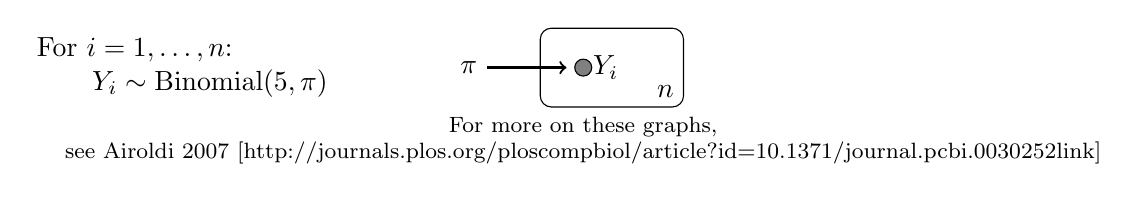
\begin{tikzpicture}[x = .15\textwidth, y = .5cm]
\node[align = left] at (-1,0) {
For $i = 1,\dots,n$: \\
$\qquad Y_i\sim \text{Binomial}(5, \pi)$
};
\draw[rounded corners] (1.5,-1) rectangle (2.5,1);
\node[circle, scale = .65, draw = black, fill = gray] (Y) at (1.8,0) {};
\node[anchor = west] at (Y) {$Y_i$};
\node[anchor = south east, align = right] at (2.5,-1) {$n$};
\node (pi) at (1,0) {$\pi$};
\draw[->, thick, shorten >= .1cm] (pi) -- (Y);
\node[font=\footnotesize, align = center, anchor = north] at (1.8,-1) {For more on these graphs, \\ see Airoldi 2007 [\href{http://journals.plos.org/ploscompbiol/article?id=10.1371/journal.pcbi.0030252}{link}]};
\end{tikzpicture}
\end{center}
}
\end{frame}

\begin{frame}
\begin{Large}We \bgreen{assume:}\end{Large} \vskip .2cm
\begin{itemize}
\item Response is binomial, with each paper independent
\item All submissions from all students having the same probability $\pi$ of success.
\end{itemize} \vskip .5cm
\begin{Large}From the data, we \bgreen{learn}:\end{Large} \vskip .2cm
\begin{itemize}
\item The value of the parameter $\hat \pi$ under which the observed data would be most likely.
\end{itemize}
\end{frame}

\begin{frame}{Binomial likelihood}
\begin{center}
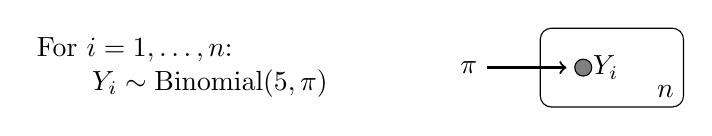
\begin{tikzpicture}[x = .15\textwidth, y = .5cm]
\node[align = left] at (-1,0) {
For $i = 1,\dots,n$: \\
$\qquad Y_i\sim \text{Binomial}(5, \pi)$
};
\draw[rounded corners] (1.5,-1) rectangle (2.5,1);
\node[circle, scale = .65, draw = black, fill = gray] (Y) at (1.8,0) {};
\node[anchor = west] at (Y) {$Y_i$};
\node[anchor = south east, align = right] at (2.5,-1) {$n$};
\node (pi) at (1,0) {$\pi$};
\draw[->, thick, shorten >= .1cm] (pi) -- (Y);
\end{tikzpicture}
\end{center}
What is the likelihood of $\pi$ given one $y_i$?
\onslide<2->{$$L(\pi\mid y_i) = \P(y_i\mid \pi) = \left(\begin{matrix}5 \\ y_i\end{matrix}\right)\pi^{y_i}(1-\pi)^{5-y_i}$$}
\onslide<3->{What is the likelihood of $\pi$ given all $n$ observations?}
\begin{center}
\begin{tikzpicture}
\node at (0,0) {$\begin{aligned}
\onslide<4->{L(\pi\mid \vec{y}) = \P(\vec{y}\mid \pi) = \P(y_1,\dots,y_n\mid \pi)}
\onslide<5->{&= \prod_{i=1}^n \P(y_i\mid \pi)} \\
\onslide<6->{&=\prod_{i=1}^n \left(\begin{matrix}5 \\ y_i\end{matrix}\right)\pi^{y_i}(1-\pi)^{5-y_i}}
\end{aligned}$};
\onslide<5->{
\node[olive,font=\footnotesize] at (1.25,1.5) {Assumes independence};
\draw[olive,->, thick] (1.25,1.3) -- (1.25,.9);
}
\end{tikzpicture}
\end{center}
\end{frame}

\begin{frame}{Review of log rules}
$$\begin{aligned}
\log(ab) &= \log(a) + \log(b) \\
\log(e^a) &= a
\end{aligned}$$
\end{frame}

\begin{frame}{$\ell(\pi\mid y_1,\dots,y_n)$: Products into sums}
$$\begin{aligned}
\ell(\pi\mid y_1,\dots,y_n) &= \pause \log L(\pi\mid y_1,\dots,y_n) \\
&= \pause \log \prod_{i=1}^n \left(\begin{matrix}5 \\ y_i\end{matrix}\right)\pi^{y_i}(1-\pi)^{5-y_i} \\
&\text{Apply rules of the log to turn products into sums} \\
&=\pause \sum_{i=1}^n \log\left(\left(\begin{matrix}5 \\ y_i\end{matrix}\right)\pi^{y_i}(1-\pi)^{5-y_i}\right) \\
&=\pause \sum_{i=1}^n \left(\log\left(\begin{matrix}5 \\ y_i\end{matrix}\right) + y_i\log(\pi) + (5 - y_i)\log(1-\pi)\right)
\end{aligned}$$
\end{frame}

\begin{frame}{$\ell(\pi\mid y_1,\dots,y_n)$: Remove constants}
$$\begin{aligned}
\ell(\pi\mid y_1,\dots,y_n) &=
	\sum_{i=1}^n \left(
	\only<1-1>{\black{\log\left(\begin{matrix}5 \\ y_i\end{matrix}\right)}}
	\only<2-| handout:0>{\blue{\log\left(\begin{matrix}5 \\ y_i\end{matrix}\right)}}
	 + y_i\log(\pi) + (5 - y_i)\log(1-\pi)\right) \\ \pause
&\text{Pull the first term out of the sum} \\
&= \pause \blue{\sum_{i=1}^n \log\left(\begin{matrix}5 \\ y_i\end{matrix}\right)} + \sum_{i=1}^n \left(y_i\log(\pi) + (5 - y_i)\log(1-\pi)\right) \\
&\text{Drop the constant which does not involve $\pi$} \\
&= \pause \sum_{i=1}^n \left(y_i\log(\pi) + (5 - y_i)\log(1-\pi)\right) + \text{constant}
\end{aligned}$$
\end{frame}

\begin{frame}{$\ell(\pi\mid y_1,\dots,y_n)$: Collect terms involving data}
$$\begin{aligned}
\only<1-5>{\black{\ell(\pi\mid y_1,\dots,y_n)}}
\only<6-| handout:0>{\blue{\ell(\pi\mid y_1,\dots,y_n)}} 
&= \sum_{i=1}^n \left(y_i\log(\pi) + (5 - y_i)\log(1-\pi)\right) \\
&= \pause \log \pi \sum_{i=1}^n y_i + 5n\log(1-\pi) - \log (1-\pi)\sum_{i=1}^n y_i \\
&= \pause 
	\only<1-3,6->{\black{(\log \pi - \log[1-\pi])}}
	\only<4-5| handout:0>{\blue{(\log \pi - \log[1-\pi])}}
	\sum_{i=1}^n y_i + 5n\log(1-\pi)  \\
\onslide<4->{&\text{Simplify by rules of logs} \\}
\only<1-4| handout:0>{
&\white{=\log \left(\frac{\pi}{1 - \pi}\right)\sum_{i=1}^n y_i+ 5n\log(1-\pi)}
}
\only<5->{
&\only<5-5| handout:0>{=\blue{\log \left(\frac{\pi}{1 - \pi}\right)}\sum_{i=1}^n y_i+ 5n\log(1-\pi)}
	\only<6->{=\blue{\log \left(\frac{\pi}{1 - \pi}\right)\sum_{i=1}^n y_i+ 5n\log(1-\pi)}}
}
\end{aligned}$$
\onslide<6->{\centering \Large \bblue{We're finished!}}
\end{frame}

\begin{frame}{Sufficient statistics}
The data $y_1,\dots,y_n$ only enter the likelihood through their \bgreen{sum}!
$$\ell(\pi\mid y_1,\dots,y_n) = \log \left(\frac{\pi}{1 - \pi}\right)\green{\sum_{i=1}^n y_i}+ 5n\log(1-\pi)$$
We call $\sum_{i=1}^n y_i$ a \bgreen{sufficient statistic}: it provides sufficient information to compute the likelihood.

\bblue{Think, Pair, Share:}
\begin{enumerate}
\onslide<2->{\item We can compute the likelihood only knowing the total number of graduate student submissions that are given R\&Rs. Can you explain this?
}
\onslide<3->{
\begin{itemize}
\item Since we assumed every submission had the same probability of success, it's like we had 5n Bernoulli trials. There is no need to distinguish who submitted them!
\end{itemize}
}
\onslide<2->{\item Why might we want to work with sufficient statistics rather than the full data?
}
\onslide<3->{
\begin{itemize}
\item Sufficient statistics can save disk space in more complex problems - no need to store all the data!
\end{itemize}
}
\end{enumerate}
\end{frame}

\section{Calculus review}
\tcframe

\begin{frame}{Calculus review: Derivatives}
Suppose we have a function
$$f(x) = x - x^2 + \log(x) + \log(3x^2)$$
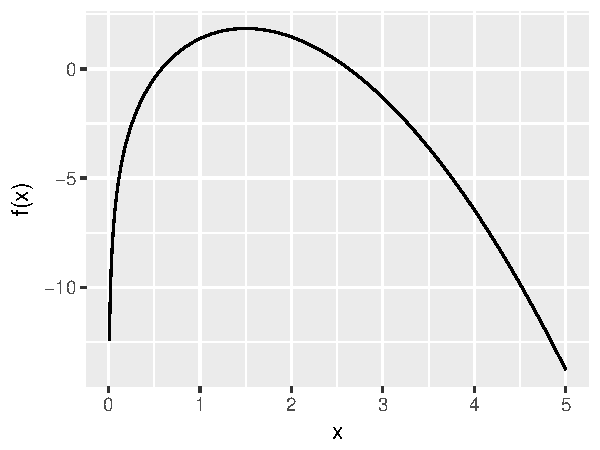
\includegraphics[width = .5\textwidth]{figs/ToMaximize.pdf} \\
What is the derivative? \pause \bgreen{It is the slope.}
\end{frame}

\begin{frame}{Calculus review: Derivatives}
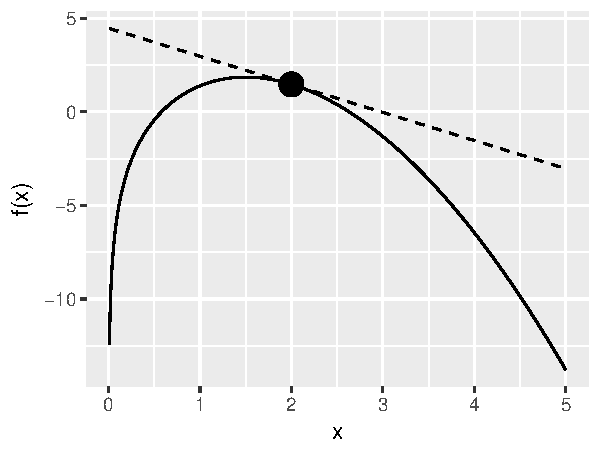
\includegraphics[width = .8\textwidth]{figs/ToMaximize2.pdf} \\
\end{frame}

\begin{frame}{Calculus review: A few derivative rules}
$$\begin{aligned}
\frac{\partial}{\partial x} x^a &= ax^{a-1} \\
\frac{\partial}{\partial x} \log x &= \frac{1}{x} \\
\frac{\partial}{\partial x} f(x) &\text{ is often denoted }f'(x) \\
\frac{\partial}{\partial x} f(g[x]) &= f'(g[x])g'(x) \text{ (often called the chain rule)} \\
\end{aligned}$$
\end{frame}

\begin{frame}{Calculus review: Derivatives}
\bblue{Check for understanding:}
$$f(x) = x - x^2 + \log(x) + \log(3x^2)$$
The derivative is
$$\begin{aligned}
\frac{\partial}{\partial x} f(x) &= \pause 1 - \pause 2x + \pause \frac{1}{x} + \pause \frac{6x}{3x^2} \\
&= \pause 1 - 2x + \frac{1}{x} + \frac{2}{x} \\
&= 1 - 2x + \frac{3}{x}
\end{aligned}$$
Let's evaluate the derivative at $x = 2$ \pause \\
$$f'(2) = 1 - 2(2) + \frac{3}{2} = -1.5$$
\end{frame}

\begin{frame}{Calculus review: Maximizing a function}
$$\begin{aligned}
f(x) &= x - x^2 + \log(x) + \log(3x^2) \\
f'(x) &= 1 - 2x + \frac{3}{x}
\end{aligned}$$
How do we maximize this? \pause \vskip 1cm
Set the derivative equal to 0 and solve! \pause \vskip 1cm
(Then check that you find a maximum) 
\end{frame}

\begin{frame}{Calculus review: Maximizing a function}
\centering 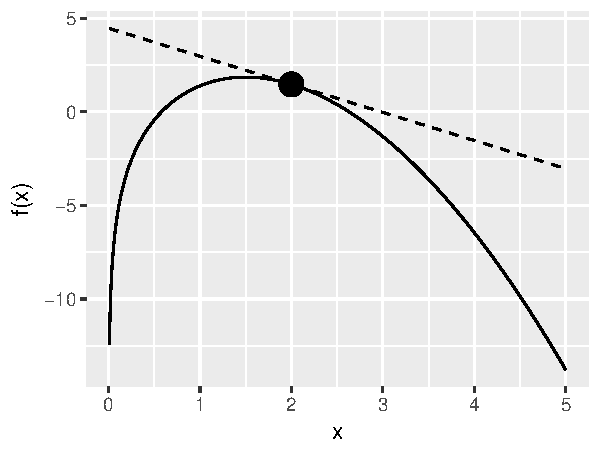
\includegraphics[width = .8\textwidth]{figs/ToMaximize2.pdf}
\end{frame}

\begin{frame}{Calculus review: Maximizing a function}
\centering 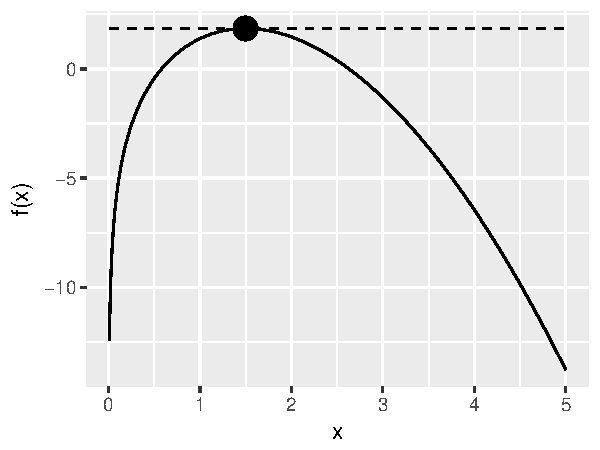
\includegraphics[width = .8\textwidth]{figs/ToMaximize3.pdf}
\end{frame}

\begin{frame}{Calculus review: Maximizing a function}
Set the derivative equal to 0
\begin{center}
\begin{tikzpicture}[x = \textwidth, y = \textheight]
\node[anchor = south west] at (0,0) {$\begin{aligned}
f'(x^*) &= 0 \\
1 - 2x^* + \frac{3}{x^*} &= 0  \pause \pause \\
\frac{3}{x^*} &= 2x^* - 1 \pause  \\
3 &= 2x^{*2} - x^* \pause  \\
0 &= 2x^{*2} - x^* - 3 \pause  \\
0 &= 2x^{*2} - x^* - 3  \pause \\
0 &= (2x^* - 3)(x^* + 1)  \pause \\
x^* &= \{-1, 1.5\}
\end{aligned}$};
\onslide<2->{
\draw[->, dashed, olive, rounded corners, line width = 1.5pt] (0,.45) rectangle (1,.63);
\node[anchor = north east, olive, align = right, font = \normalsize] at (1, .63) {\bgreen{Useful skill:}\\Set derivative equal to 0};
}
\onslide<3->{
\node[anchor = east, rotate = -20, align = center, blue, font =\bf, draw = blue, line width = 1.5pt] at (.8,.25) {Algebra:\\Not important};
}
\end{tikzpicture}
\end{center}
These are our \textbf{critical values}.
\end{frame}

\begin{frame}{Calculus review: Second derivative}
The second derivative captures the curvature of the function.
$$\begin{aligned}
f''(x) &= \frac{\partial}{\partial x} 1 - 2x + \frac{3}{x} \pause \\
&= \frac{\partial}{\partial x} 1 - 2x +3x^{-1} \pause \\
&= -2 - 3x^{-2} \pause  \\
&= -2 - \frac{3}{x^2}
\end{aligned}$$ \pause
\begin{center}
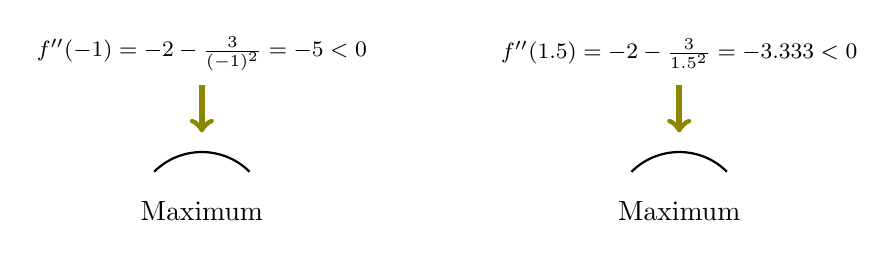
\begin{tikzpicture}[x = .25\textwidth, y = 1cm]
\node[font = \footnotesize] (negative) at (-1,2) {$f''(-1) = -2 - \frac{3}{(-1)^2} = -5 < 0$};
\node[font = \footnotesize] (negative2) at (1,2) {$f''(1.5) = -2 - \frac{3}{1.5^2} = -3.333 < 0$};
\draw[->, olive, line width = 2pt] (-1,1.6) -- (-1, 1);
\draw[->, olive, line width = 2pt] (1,1.6) -- (1, 1);
\draw[thick] (-1.2,.5) to[bend left = 45] (-.8, .5);
\draw[thick] (.8, .5) to[bend left = 45] (1.2,.5);
\node at (-1,0) {Maximum};
\node at (1,0) {Maximum};
\end{tikzpicture}
\end{center}
\end{frame}

\section{Maximizing the likelihood}
\tcframe

\begin{frame}{Back to our example: Maximizing the log likelihood}
$$\ell(\pi\mid y_1,\dots,y_n) = (\log \pi - \log[1-\pi]) \sum_{i=1}^n y_i + 5n\log(1-\pi)$$
To maximize, \pause take the derivative and set it equal to 0! \pause
$$\begin{aligned}
\frac{\partial}{\partial \pi} \ell(\pi\mid y_1,\dots,y_n) &= \frac{\partial}{\partial \pi} (\log \pi - \log[1-\pi]) \sum_{i=1}^n y_i + 5n\log(1-\pi) \\
&= \pause \frac{\partial}{\partial\pi} (\log \pi - \log[1-\pi]) \sum_{i=1}^n y_i + 5n\log(1-\pi) \\
&= \pause \frac{1}{\pi}\sum_{i=1}^n y_i + \frac{\sum_{i=1}^n y_i - 5n}{1-\pi} \\
\end{aligned}$$
\end{frame}

\begin{frame}
\begin{center}
\begin{tikzpicture}[x = \textwidth, y = \textheight]
\node[anchor = south west] at (0,0) {$\begin{aligned}
0 &= \frac{1}{\pi^*}\sum_{i=1}^n y_i + \frac{\sum_{i=1}^n y_i - 5n}{1-\pi^*} \\ \pause \pause
\frac{5n - \sum_{i=1}^n y_i}{1-\pi^*} &= \frac{1}{\pi^*}\sum_{i=1}^n y_i \\ \pause 
(5n - \sum_{i=1}^n y_i)\pi^* &= (1-\pi^*)\sum_{i=1}^n y_i \\ \pause
5n \pi^* &= \sum_{i=1}^n y_i \\ \pause
\pi^* &= \frac{\sum_{i=1}^n y_i}{5n} \\
\end{aligned}$};
\onslide<2->{
\draw[->, dashed, olive, rounded corners, line width = 1.5pt] (0,.55) rectangle (1,.7);
\node[anchor = north east, olive, align = right, font = \footnotesize] at (1, .7) {\bgreen{Useful skill:}\\Set derivative\\equal to 0};
}
\onslide<3->{
\node[anchor = east, rotate = -20, align = center, blue, font =\bf, draw = blue, line width = 1.5pt] at (.85,.35) {Algebra:\\Not important};
}
\end{tikzpicture}
\end{center}
\onslide<7->{This $\pi^*$ such that $\ell'(\pi\mid y)=0$ is the \bgreen{critical value}.} \onslide<8>{Is it a max?}
\end{frame}

\begin{frame}{Back to our example: Maximizing the log likelihood}
\begin{center}
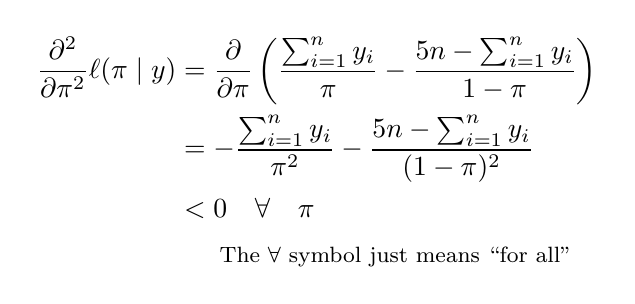
\begin{tikzpicture}
\node[anchor = south] at (0,0) {$\begin{aligned}
\frac{\partial^2}{\partial \pi^2} \ell(\pi\mid y) &= \frac{\partial}{\partial \pi} \left(\frac{\sum_{i=1}^n y_i}{\pi} - \frac{5n - \sum_{i=1}^n y_i}{1-\pi}\right) \\ \pause
&= -\frac{\sum_{i=1}^n y_i}{\pi^2} - \frac{5n - \sum_{i=1}^n y_i}{(1-\pi)^2} \\ \pause
&<0\hspace{10pt}\forall\hspace{10pt}\pi \pause
\end{aligned}$};
\onslide<3->{\node[anchor = north, font = \footnotesize] at (1,0) {The $\forall$ symbol just means ``for all''};}
\end{tikzpicture}
\end{center}
\onslide<4->{
Since the first derivative is 0 and the second derivative is negative, the critical value $\pi^* = \frac{\sum_{i=1}^n y_i}{5n}$ is a maximum.
$$\hat \pi_\text{MLE} = \frac{\sum_{i=1}^n y_i}{5n}$$
}
\end{frame}

\begin{frame}[fragile]{Plotting the log likelihood}
$$\ell(\pi\mid y_1,\dots,y_n) = (\log \pi - \log[1-\pi]) \sum_{i=1}^n y_i + 5n\log(1-\pi)$$
Let's define a function in R that returns the log likelihood given a vector \texttt{y} \pause

\begin{scriptsize}
\begin{semiverbatim}
log.lik <- function(pi,y) \{
     (log(pi) - log(1 - pi)) * sum(y) + 5 * length(y) * log(1 - pi)
\}
\end{semiverbatim}
\end{scriptsize}

\end{frame}

\begin{frame}[fragile]{Plotting the log likelihood}
Define some data and make a plot.
\begin{center}
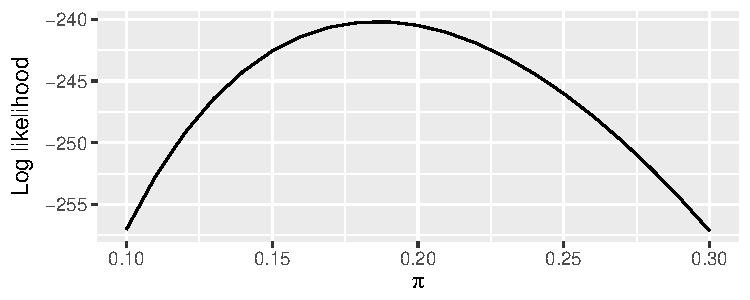
\includegraphics[width = .8\textwidth]{figs/LogLik1.pdf}
\end{center}
\begin{small}
\begin{semiverbatim}
y <- rbinom(100,5,.2) \pause
data.frame(pi = seq(0.1,0.3,0.01)) \%>\% \pause
  mutate(`Log likelihood` = log.lik(pi,y)) \%>\% \pause
  ggplot(aes(x = pi, y = `Log likelihood`)) + \pause
  geom_line() + \pause
  scale_x_continuous(name = expression(pi))
\end{semiverbatim}
\end{small}
\end{frame}

\begin{frame}[fragile]{Finding the maximum numerically}

\begin{semiverbatim}
> y <- rbinom(100,5,.2)
> optimize(f = log.lik,
+          interval = c(0,1),
+          maximum = T,
+          y = y)
$maximum
[1] 0.1860007

$objective
[1] -240.1853
\end{semiverbatim}
\end{frame}

\section{Invariance}
\tcframe

\begin{frame}{Invariance of the MLE}

\begin{theorem}[King Sec. 4.4, Casella \& Berger Thm 7.2.10]
\normalfont If $\hat\theta_\text{MLE}$ is the MLE for $\theta$, then for any function $g(\theta)$ the MLE of $g(\theta)$ is $g(\hat\theta_\text{MLE})$.
\end{theorem} \vskip .2cm
\bblue{Application:} If we knew the true $\pi = \P(\text{R\&R})$, what would be the probability of getting at least 1 R\&R out of 5 submissions? \pause
$$\begin{aligned}
\P(\text{At least 1 R\&R out of 5 submissions}) &= 1 - \P(5\text{ rejections}) \\
&= 1 - (1 - \pi)^5 = g(\pi)\end{aligned}$$
\bgreen{Question:} If we have $\hat\pi_\text{MLE} = 0.186$, what is $\hat\tau_\text{MLE} = \widehat{g(\pi)}_\text{MLE}$?
\end{frame}

\begin{frame}

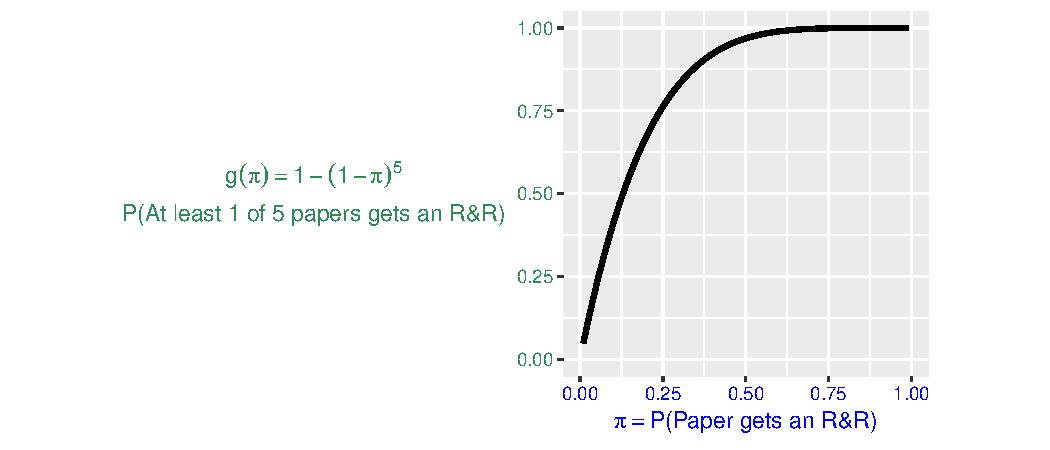
\includegraphics[width = .8\textwidth]{figs/g_pi} \\ \pause
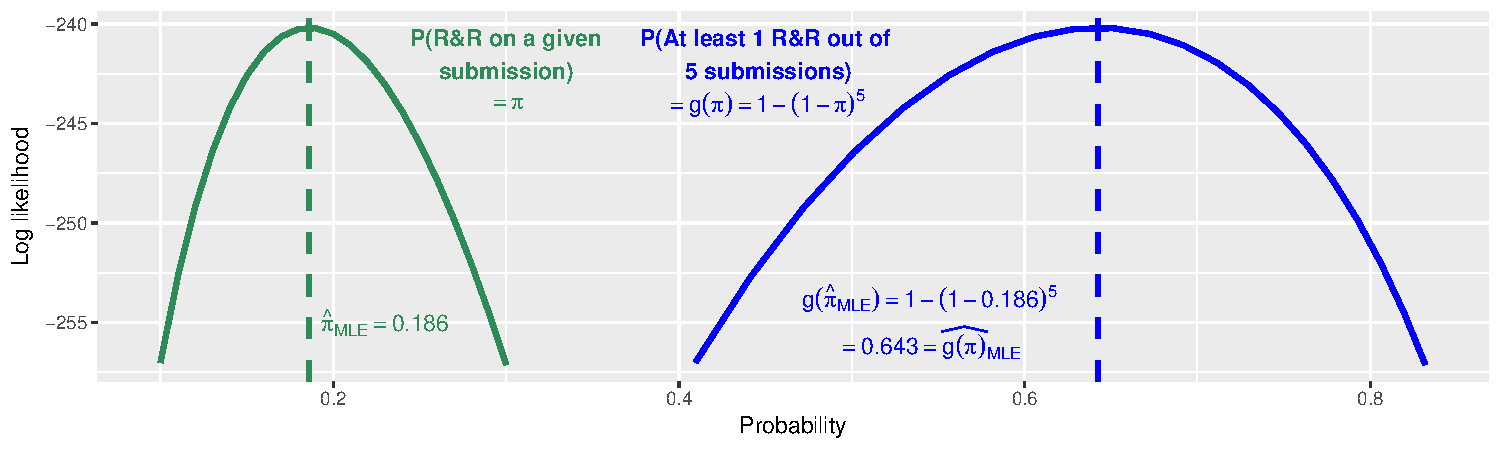
\includegraphics[width = \textwidth]{figs/LogLik_both}

\end{frame}

\section{Uncertainty}
\tcframe

\begin{frame}{Uncertainty: Curvature at the maximum}
We can estimate uncertainty from the curvature of $\ell$ around the MLE.

\begin{center}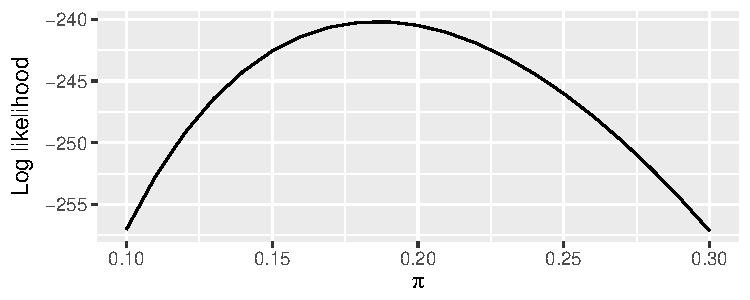
\includegraphics[width = .6\textwidth]{figs/LogLik1.pdf} \end{center}
\end{frame}

\begin{frame}{Uncertainty: Curvature at the maximum}
The negative of the curvature at the MLE is referred to as the \href{https://en.wikipedia.org/wiki/Fisher_information}{\bgreen{Fisher information}}. \pause
$$\mathcal{I}_n(\theta) = -\E\left(\frac{\partial^2}{\partial\theta^2}\ell(\theta\mid y)\bigg\rvert_{\theta = \theta_\text{MLE}}\right)$$ \pause
The \bgreen{variance of the MLE} is the inverse of the Fisher information:
$$\V(\hat\theta_{\text{MLE}}) = \frac{1}{\mathcal{I}_n(\theta)}$$ \pause
The expectation is taken over the distribution of possible samples $y$, evaluated at the true $\theta$. We often estimate by using our one sample to calculate the \bgreen{observed fisher information} at $\hat\theta_\text{MLE}$.
\begin{center}

\begin{tikzpicture}
\node[anchor = east] (eq) at (0,0) {$\hat\V\left(\hat\theta_{\text{MLE}}\right) = \bigg(\hat{\mathcal{I}}_n(\theta)\bigg)^{-1}\bigg\rvert_{\theta = \hat\theta_\text{MLE}}$};
\node[anchor = west, olive, align = center, font = \footnotesize] (explanation) at (0,0) {Read ``evaluated at\\$\theta = \hat\theta_\text{MLE}$''};
\draw[->, thick, olive] (0,.25) to[bend right] (-.7,-.1);
\end{tikzpicture}
\end{center}
\end{frame}

\begin{frame}{Uncertainty: Curvature at the maximum}
What is the uncertainty of our $\hat\pi_\text{MLE}$? We already calculated:
$$\begin{aligned}
\frac{\partial^2}{\partial \pi^2} \ell(\pi\mid y) 
	&= -\frac{\sum_{i=1}^n y_i}{\pi^2} - \frac{5n - \sum_{i=1}^n y_i}{(1-\pi)^2}
\end{aligned}$$
$$\hat\pi_\text{MLE} = \frac{\sum_{i=1}^n y_i}{5n} = \frac{\bar{y}}{5}$$
From the prior slide,
$\hat\V\left(\hat\theta_{\text{MLE}}\right) = \bigg(\hat{\mathcal{I}}_n(\theta)\bigg)^{-1}\bigg\rvert_{\theta = \hat\theta_\text{MLE}} = -\left[\frac{\partial^2}{\partial\theta^2}\ell(\theta\mid y)\right]^{-1}\bigg\rvert_{\theta = \hat\theta_\text{MLE}}$ \vskip .5cm
\bblue{Think, Pair, and Share:} What would be the first step to write a formula for $\hat\V\left(\hat\pi_{\text{MLE}}\right)$?
\end{frame}

\begin{frame}{Uncertainty: Curvature at the maximum}
\begin{footnotesize}

\begin{tikzpicture}[x = \textwidth, y = \textheight]
\node[anchor = south west] at (0,0) {$\begin{aligned}
\hat{V}\left(\hat\pi_\text{MLE}\right) &= -\left(
	-\frac{
		\sum_{i=1}^n y_i
	}{
		\hat\pi_\text{MLE}^2
	} - \frac{
		5n - \sum_{i=1}^n y_i
	}{
		(1-\hat\pi_\text{MLE})^2
	}\right)^{-1} \\ \pause
&= -\left(-\frac{
		\sum_{i=1}^n y_i
	}{
		\left(\frac{\sum_{i=1}^n y_i}{5n}\right)^2
	} - \frac{
		5n - \sum_{i=1}^n y_i
	}{
		\left(1-\frac{\sum_{i=1}^n y_i}{5n}\right)^2
	}\right)^{-1} \\ \pause \pause
&= -\left(
	-\frac{
		(5n)^2\left(\sum_{i=1}^n y_i\right)
	}{
		\left(\sum_{i=1}^n y_i\right)^2
	} - \frac{
		(5n)^2\left(5n - \sum_{i=1}^n y_i\right)
	}{
		\left(5n-\sum_{i=1}^n y_i\right)^2
	}\right)^{-1} \\ \pause
&= \frac{1}{(5n)^2}\left(
	\frac{
		1
	}{
		\sum_{i=1}^n y_i
	} + \frac{
		1
	}{
		5n-\sum_{i=1}^n y_i
	}\right)^{-1} \\ \pause
&= \frac{1}{(5n)^2}\left(
	\frac{
		5n-\sum_{i=1}^n y_i + \sum_{i=1}^n y_i
	}{
		\left(\sum_{i=1}^n y_i\right)\left(5n-\sum_{i=1}^n y_i\right)
	}\right)^{-1} \\  \pause
&= \frac{1}{(5n)^2}\left(
	\frac{
		\left(\sum_{i=1}^n y_i\right)\left(5n-\sum_{i=1}^n y_i\right)
	}{
		5n
	}\right) \\ \pause
&=  \frac{1}{5n}
	\left(\frac{\sum_{i=1}^n y_i}{5n}\right)
	\left(\frac{5n-\sum_{i=1}^n y_i}{5n}\right)
\end{aligned}$};
\onslide<3->{
\draw[->, dashed, olive, rounded corners, line width = 1.5pt] (0,.59) rectangle (1,.9);
\node[anchor = north east, olive, align = right, font = \normalsize] at (1, .9) {\bgreen{Useful skill:}\\Plug a particular\\estimate into a\\general MLE formula};
}
\onslide<4->{
\node[anchor = east, rotate = -20, align = center, blue, font =\bf, draw = blue, line width = 1.5pt] at (1,.4) {Algebra:\\Not important};
}
\end{tikzpicture}
\end{footnotesize}
\end{frame}

\begin{frame}{Uncertainty result: Building intuition}
\bblue{Question:} Does anyone have intuition about our result?
\begin{center}
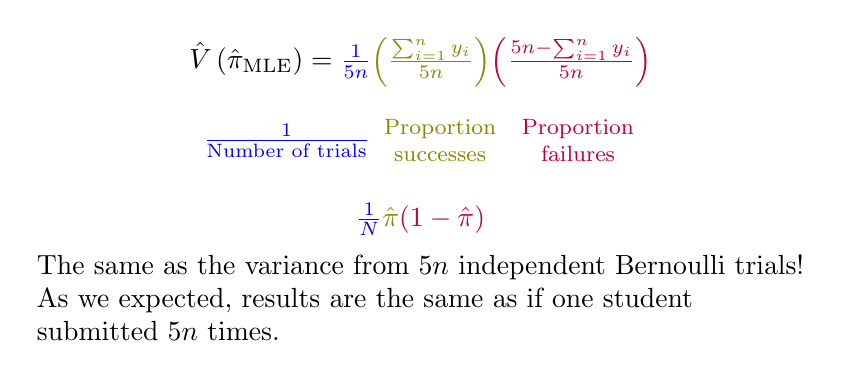
\begin{tikzpicture}
\node at (0,0) {$\hat{V}\left(\hat\pi_\text{MLE}\right) = \blue{\frac{1}{5n}}
	\green{\left(\frac{\sum_{i=1}^n y_i}{5n}\right)}
	\purple{\left(\frac{5n-\sum_{i=1}^n y_i}{5n}\right)}$};
\onslide<2->{
\node[blue] at (-1.7,-1) {$\frac{1}{\text{Number of trials}}$};
\node[olive,align=center,font=\footnotesize] at (0.25,-1) {Proportion\\successes};
\node[purple,align=center,font=\footnotesize] at (2,-1) {Proportion\\failures};
\node at (0,-2) {$\blue{\frac{1}{N}}\green{\hat{\pi}}\purple{(1-\hat{\pi})}$};
}
\onslide<3->{
\node[align=left] at (0, -3) {The same as the variance from $5n$ independent Bernoulli trials!\\As we expected, results are the same as if one student\\submitted $5n$ times.};
}
\end{tikzpicture}
\end{center}
\begin{large}
\onslide<4->{
\bgreen{Lesson:} A story tying your model to a simpler, known result can help you build confidence in your derivation.
}
\end{large}
\end{frame}

\section[Tests]{Hypothesis tests: Wald, score, and likelihood ratio}
\tcframe

\begin{frame}{Hypothesis tests\footnote{These tests can be generalized to the null hypothesis $H_0: h(\vec\theta\,) = \vec{c}$, where $h$ is a function that maps the vector $\vec\theta\in\mathbb{R}^p$ to a vector of constraints $c\in \mathbb{R}^k$.}}
Suppose we want to test the null hypothesis that a subset of the coefficients are zero.
$$\vec\beta = \begin{bmatrix} \vec\beta_A \\ \vec\beta_B \end{bmatrix},\qquad H_0: \vec\beta = \vec\beta_0 \equiv \begin{bmatrix} \vec{0} \\ \vec\beta_B \end{bmatrix}$$
There are three main methods for conducting this test.

\begin{center}
\scalebox{.7}{
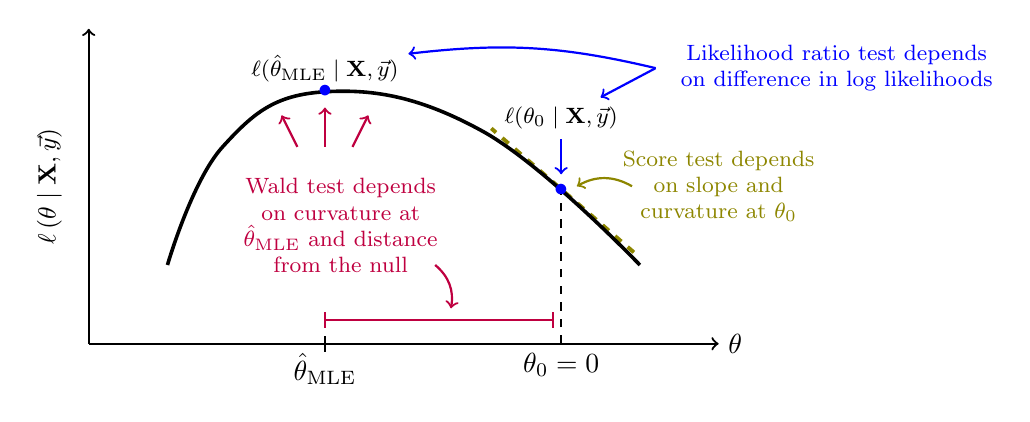
\begin{tikzpicture}
% Score test
\node[olive, font = \footnotesize,align = center] at (5, 2) {Score test depends\\on slope and\\curvature at $\theta_0$};
\draw[olive, line width = 1.4pt, dashed, rotate = 49] (3.45,-2.2) -- (3.45,.2);
\draw[->, thick, olive] (3.9,2) to[bend right] (3.2,2);
% Wald test
\node[purple, font = \footnotesize,align = center] at (0.2,1.5) {Wald test depends\\on curvature at\\$\hat\theta_\text{MLE}$ and distance\\from the null};
\draw[->, thick, purple] (0,2.5) -- (0,3);
\draw[->, thick, purple] (-.35,2.5) -- (-.55,2.9);
\draw[->, thick, purple] (.35,2.5) -- (.55,2.9);
\draw[-, thick, purple] (0,.3) -- (2.9,.3);
\draw[-, thick, purple] (0,.2) -- (0,.4);
\draw[-, thick, purple] (2.9,.2) -- (2.9,.4);
\draw[->, thick, purple] (1.4,1) to[bend left] (1.6,.45);
% Curve
\draw[line width = 1.3] plot [smooth,tension=.7] coordinates {(-2,1) (-1.3,2.5) (0,3.2) (2,2.7) (4,1)};
% MLE
\node[anchor = south,font = \footnotesize] (mleLabel) at (0,3.2) {$\ell(\hat\theta_\text{MLE}\mid \mathbf{X},\vec{y})$};
\node[fill=none,blue] (mle) at (0,3.2) {$\bullet$};
% Null hypothesis
\node[anchor = south,font = \footnotesize] (nullLabel) at (3,2.6) {$\ell(\theta_0\mid \mathbf{X},\vec{y})$};
\node[fill=none,blue] (null) at (3,1.95) {$\bullet$};
\draw[->, thick, blue] (nullLabel) -- (null);
% Likelihood ratio test
\node[blue, font = \footnotesize,align = center] at (6.5,3.5) {Likelihood ratio test depends\\on difference in log likelihoods};
\draw[->, thick, blue] (4.2,3.5) to[bend right = 10] (mleLabel);
\draw[->, thick, blue] (4.2,3.5) -- (nullLabel);
% Axes
\draw[->, thick] (-3, 0) -- (-3, 4);
\draw[->, thick] (-3, 0) -- (5, 0);
\node[anchor=north] at (0,0) {$\hat\theta_\text{MLE}$};
\draw[-, thick] (0, -.1) -- (0, .1);
\node[anchor=west] at (5,0) {$\theta$};
\node[rotate=90] at (-3.5,2) {\small $\ell\left(\theta\mid \mathbf{X},\vec{y}\right)$};
\node[anchor=north] at (3,0) {$\theta_0=0$};
\draw[thick, dashed] (3,0) -- (3,1.9);
\end{tikzpicture}
}
\end{center}
\end{frame}

\begin{frame}{Wald test}
The \bgreen{Wald test} relies on the asymptotic normality of $\hat\beta_\text{MLE}$:
\begin{center}
\scalebox{.9}{
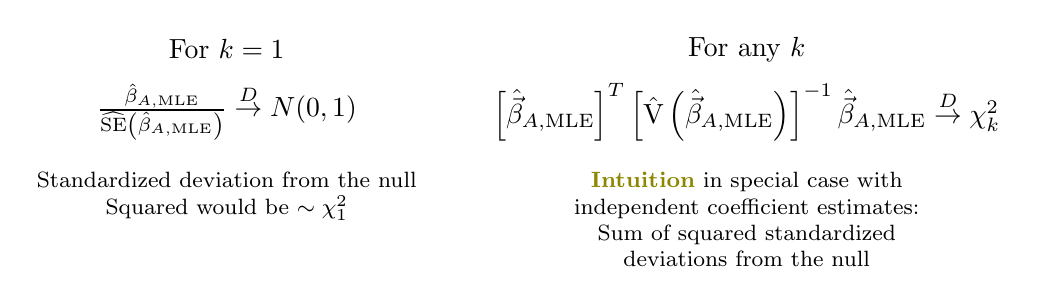
\begin{tikzpicture}[x = 1.3in, y = .8cm]
\node at (-1,1) {For $k=1$};
\node at (1,1) {For any $k$};
\node at (-1,0) {$\frac{\hat\beta_{A,\text{MLE}}}{\widehat{\text{SE}}\left(\hat\beta_{A,\text{MLE}}\right)} \stackrel{D}{\rightarrow} N(0,1)$};
\node at (1,0) {$\left[\hat{\vec\beta}_{A,\text{MLE}}\right]^T
	\left[\hat\V\left(\hat{\vec{\beta}}_{A,\text{MLE}}\right)\right]^{-1}
	\hat{\vec\beta}_{A,\text{MLE}}
	\stackrel{D}{\rightarrow} \chi^2_k$};
\node[align=center,anchor=north,font=\footnotesize] at (-1,-.8) {Standardized deviation from the null\\Squared would be $\sim \chi^2_1$};
\node[align=center,anchor=north,font=\footnotesize] at (1,-.8) {\bgreen{Intuition} in special case with\\independent coefficient estimates:\\Sum of squared standardized\\deviations from the null};
\end{tikzpicture}
}\vskip .2cm
\scalebox{.7}{
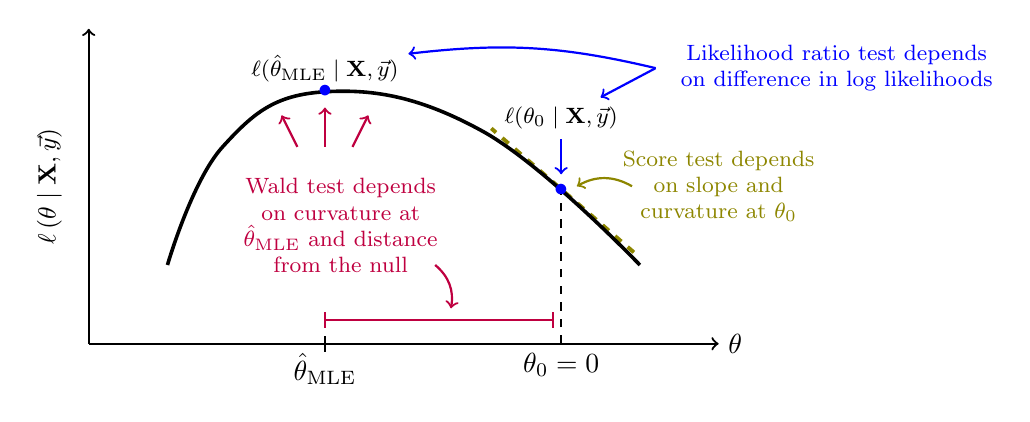
\begin{tikzpicture}
% Score test
\node[olive, font = \footnotesize,align = center] at (5, 2) {Score test depends\\on slope and\\curvature at $\theta_0$};
\draw[olive, line width = 1.4pt, dashed, rotate = 49] (3.45,-2.2) -- (3.45,.2);
\draw[->, thick, olive] (3.9,2) to[bend right] (3.2,2);
% Wald test
\node[purple, font = \footnotesize,align = center] at (0.2,1.5) {Wald test depends\\on curvature at\\$\hat\theta_\text{MLE}$ and distance\\from the null};
\draw[->, thick, purple] (0,2.5) -- (0,3);
\draw[->, thick, purple] (-.35,2.5) -- (-.55,2.9);
\draw[->, thick, purple] (.35,2.5) -- (.55,2.9);
\draw[-, thick, purple] (0,.3) -- (2.9,.3);
\draw[-, thick, purple] (0,.2) -- (0,.4);
\draw[-, thick, purple] (2.9,.2) -- (2.9,.4);
\draw[->, thick, purple] (1.4,1) to[bend left] (1.6,.45);
% Curve
\draw[line width = 1.3] plot [smooth,tension=.7] coordinates {(-2,1) (-1.3,2.5) (0,3.2) (2,2.7) (4,1)};
% MLE
\node[anchor = south,font = \footnotesize] (mleLabel) at (0,3.2) {$\ell(\hat\theta_\text{MLE}\mid \mathbf{X},\vec{y})$};
\node[fill=none,blue] (mle) at (0,3.2) {$\bullet$};
% Null hypothesis
\node[anchor = south,font = \footnotesize] (nullLabel) at (3,2.6) {$\ell(\theta_0\mid \mathbf{X},\vec{y})$};
\node[fill=none,blue] (null) at (3,1.95) {$\bullet$};
\draw[->, thick, blue] (nullLabel) -- (null);
% Likelihood ratio test
\node[blue, font = \footnotesize,align = center] at (6.5,3.5) {Likelihood ratio test depends\\on difference in log likelihoods};
\draw[->, thick, blue] (4.2,3.5) to[bend right = 10] (mleLabel);
\draw[->, thick, blue] (4.2,3.5) -- (nullLabel);
% Axes
\draw[->, thick] (-3, 0) -- (-3, 4);
\draw[->, thick] (-3, 0) -- (5, 0);
\node[anchor=north] at (0,0) {$\hat\theta_\text{MLE}$};
\draw[-, thick] (0, -.1) -- (0, .1);
\node[anchor=west] at (5,0) {$\theta$};
\node[rotate=90] at (-3.5,2) {\small $\ell\left(\theta\mid \mathbf{X},\vec{y}\right)$};
\node[anchor=north] at (3,0) {$\theta_0=0$};
\draw[thick, dashed] (3,0) -- (3,1.9);
\end{tikzpicture}
}
\end{center}
\end{frame}

\begin{frame}{Likelihood ratio test}
The \bgreen{likelihood ratio test} compares nested models:
\begin{enumerate}
\item A restricted model estimating $\vec\beta_B$ and assuming $\vec\beta_A=0$ with likelihood $L^*_R$
\item An unrestricted model with likelihood $L^*$
\end{enumerate}
$$-2\log\left(\frac{L^*_R}{L^*}\right) \stackrel{D}{\rightarrow} \chi^2_k$$
\begin{footnotesize}\bgreen{Intuition:} We have more evidence in favor of the unrestricted model if the likelihood ($L^*_R$) under the restricted model is much smaller than the likelihood ($L^*$) under the unrestricted model. We need more evidence if $k$ is larger.\end{footnotesize}
\begin{center}
\scalebox{.7}{
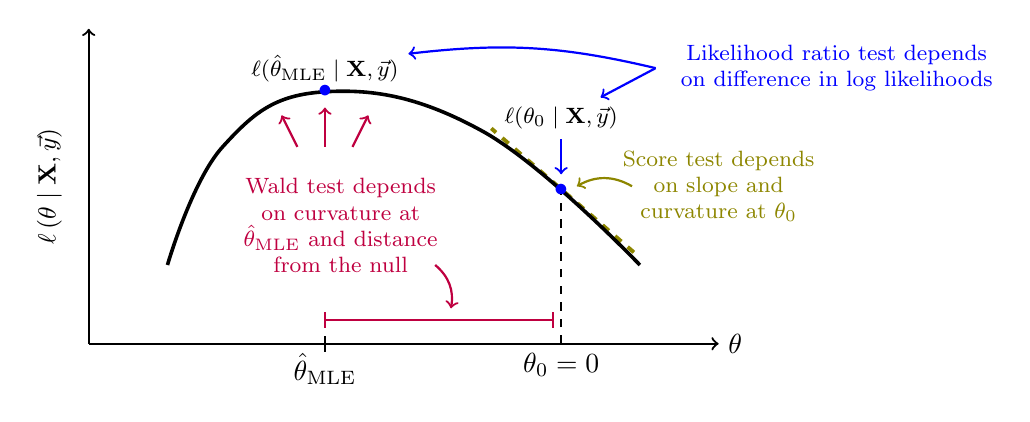
\begin{tikzpicture}
% Score test
\node[olive, font = \footnotesize,align = center] at (5, 2) {Score test depends\\on slope and\\curvature at $\theta_0$};
\draw[olive, line width = 1.4pt, dashed, rotate = 49] (3.45,-2.2) -- (3.45,.2);
\draw[->, thick, olive] (3.9,2) to[bend right] (3.2,2);
% Wald test
\node[purple, font = \footnotesize,align = center] at (0.2,1.5) {Wald test depends\\on curvature at\\$\hat\theta_\text{MLE}$ and distance\\from the null};
\draw[->, thick, purple] (0,2.5) -- (0,3);
\draw[->, thick, purple] (-.35,2.5) -- (-.55,2.9);
\draw[->, thick, purple] (.35,2.5) -- (.55,2.9);
\draw[-, thick, purple] (0,.3) -- (2.9,.3);
\draw[-, thick, purple] (0,.2) -- (0,.4);
\draw[-, thick, purple] (2.9,.2) -- (2.9,.4);
\draw[->, thick, purple] (1.4,1) to[bend left] (1.6,.45);
% Curve
\draw[line width = 1.3] plot [smooth,tension=.7] coordinates {(-2,1) (-1.3,2.5) (0,3.2) (2,2.7) (4,1)};
% MLE
\node[anchor = south,font = \footnotesize] (mleLabel) at (0,3.2) {$\ell(\hat\theta_\text{MLE}\mid \mathbf{X},\vec{y})$};
\node[fill=none,blue] (mle) at (0,3.2) {$\bullet$};
% Null hypothesis
\node[anchor = south,font = \footnotesize] (nullLabel) at (3,2.6) {$\ell(\theta_0\mid \mathbf{X},\vec{y})$};
\node[fill=none,blue] (null) at (3,1.95) {$\bullet$};
\draw[->, thick, blue] (nullLabel) -- (null);
% Likelihood ratio test
\node[blue, font = \footnotesize,align = center] at (6.5,3.5) {Likelihood ratio test depends\\on difference in log likelihoods};
\draw[->, thick, blue] (4.2,3.5) to[bend right = 10] (mleLabel);
\draw[->, thick, blue] (4.2,3.5) -- (nullLabel);
% Axes
\draw[->, thick] (-3, 0) -- (-3, 4);
\draw[->, thick] (-3, 0) -- (5, 0);
\node[anchor=north] at (0,0) {$\hat\theta_\text{MLE}$};
\draw[-, thick] (0, -.1) -- (0, .1);
\node[anchor=west] at (5,0) {$\theta$};
\node[rotate=90] at (-3.5,2) {\small $\ell\left(\theta\mid \mathbf{X},\vec{y}\right)$};
\node[anchor=north] at (3,0) {$\theta_0=0$};
\draw[thick, dashed] (3,0) -- (3,1.9);
\end{tikzpicture}
}
\end{center}
\end{frame}

\begin{frame}{Score test}
The \bgreen{score test} is based on the score function and the Fisher information evaluated at $\vec\beta_0$.
\begin{center}
\scalebox{.7}{
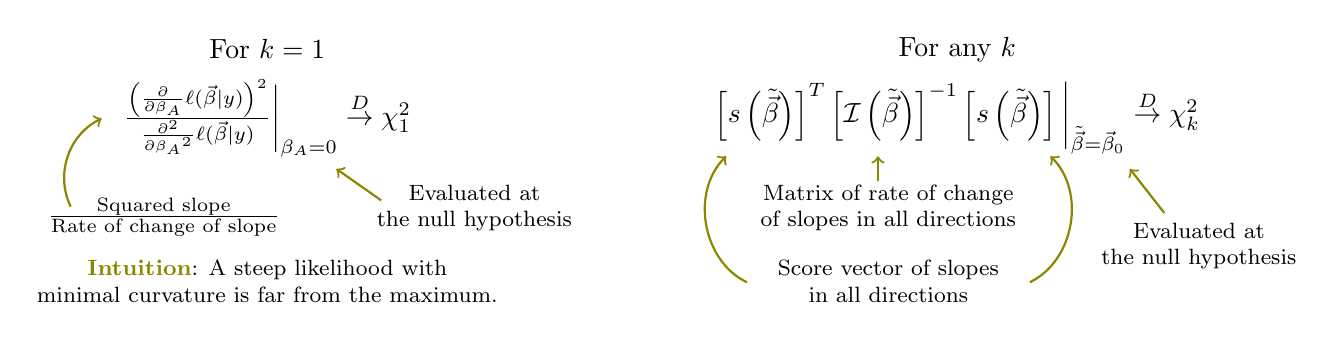
\begin{tikzpicture}[x = 1.725in, y = .8cm]
\node at (-1,1.1) {For $k=1$};
\node at (1,1.1) {For any $k$};
\node at (-1,0) {$\frac{\left(\frac{\partial}{\partial \beta_A}\ell(\vec\beta\mid y)\right) ^ 2}
	{\frac{\partial^2}{\partial {\beta_A}^2}\ell(\vec\beta\mid y)}
	\bigg\rvert_{\beta_A = 0}
	\stackrel{D}{\rightarrow} \chi^2_1$};
\node at (1,0) {$\left[s\left(\tilde{\vec\beta}\right)\right]^T
	\left[\mathcal{I}\left(\tilde{\vec\beta}\right)\right]^{-1}
	\left[s\left(\tilde{\vec\beta}\right)\right]\bigg\rvert_{\tilde{\vec\beta} = \vec\beta_0}
	\stackrel{D}{\rightarrow} \chi^2_k$};
\node[align=center,anchor=north] at (-1.3,-1.1) {$\frac{\text{Squared slope}}{\text{Rate of change of slope}}$};
\draw[->, thick, olive] (-1.57,-1.4) to[bend left = 45] (-1.48,0);
\node[align=center,anchor=north,font=\footnotesize] at (-.4,-.9) {Evaluated at\\the null hypothesis};
\draw[->, thick, olive] (-.67,-1.3) -- (-.8,-.8);
\node[align=center,anchor=north,font=\footnotesize] at (-1,-2.1) {\bgreen{Intuition}: A steep likelihood with\\minimal curvature is far from the maximum.};
\node[align=center,anchor=north,font=\footnotesize] at (.8,-.9) {Matrix of rate of change\\of slopes in all directions};
\node[align=center,anchor=north,font=\footnotesize] at (.8,-2.1) {Score vector of slopes\\in all directions};
\draw[->, thick, olive] (.39,-2.6) to[bend left = 55] (.33,-.6);
\draw[->, thick, olive] (1.21,-2.6) to[bend right = 55] (1.27,-.6);
\draw[->, thick, olive] (0.77,-1) -- (0.77,-.6);
\node[align=center,anchor=north,font=\footnotesize] at (1.7,-1.5) {Evaluated at\\the null hypothesis};
\draw[->, thick, olive] (1.6,-1.5) -- (1.5,-.8);
\end{tikzpicture}
}\vskip .2cm
\scalebox{.7}{
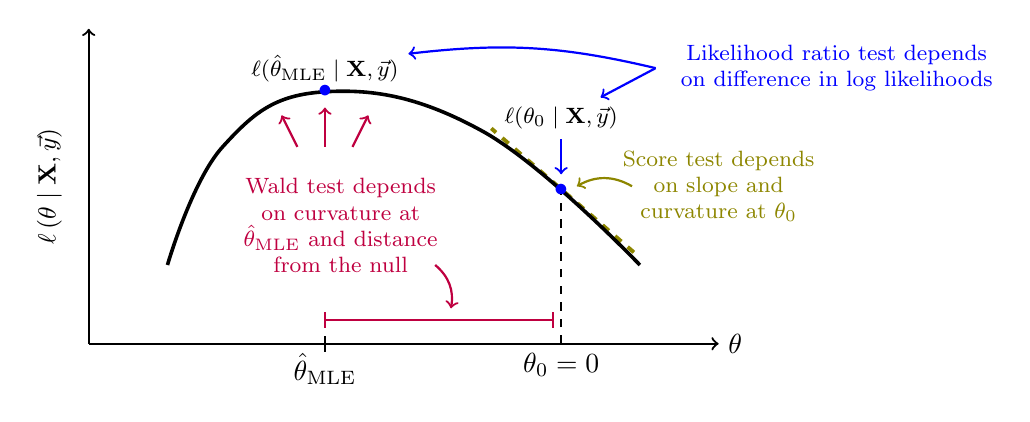
\begin{tikzpicture}
% Score test
\node[olive, font = \footnotesize,align = center] at (5, 2) {Score test depends\\on slope and\\curvature at $\theta_0$};
\draw[olive, line width = 1.4pt, dashed, rotate = 49] (3.45,-2.2) -- (3.45,.2);
\draw[->, thick, olive] (3.9,2) to[bend right] (3.2,2);
% Wald test
\node[purple, font = \footnotesize,align = center] at (0.2,1.5) {Wald test depends\\on curvature at\\$\hat\theta_\text{MLE}$ and distance\\from the null};
\draw[->, thick, purple] (0,2.5) -- (0,3);
\draw[->, thick, purple] (-.35,2.5) -- (-.55,2.9);
\draw[->, thick, purple] (.35,2.5) -- (.55,2.9);
\draw[-, thick, purple] (0,.3) -- (2.9,.3);
\draw[-, thick, purple] (0,.2) -- (0,.4);
\draw[-, thick, purple] (2.9,.2) -- (2.9,.4);
\draw[->, thick, purple] (1.4,1) to[bend left] (1.6,.45);
% Curve
\draw[line width = 1.3] plot [smooth,tension=.7] coordinates {(-2,1) (-1.3,2.5) (0,3.2) (2,2.7) (4,1)};
% MLE
\node[anchor = south,font = \footnotesize] (mleLabel) at (0,3.2) {$\ell(\hat\theta_\text{MLE}\mid \mathbf{X},\vec{y})$};
\node[fill=none,blue] (mle) at (0,3.2) {$\bullet$};
% Null hypothesis
\node[anchor = south,font = \footnotesize] (nullLabel) at (3,2.6) {$\ell(\theta_0\mid \mathbf{X},\vec{y})$};
\node[fill=none,blue] (null) at (3,1.95) {$\bullet$};
\draw[->, thick, blue] (nullLabel) -- (null);
% Likelihood ratio test
\node[blue, font = \footnotesize,align = center] at (6.5,3.5) {Likelihood ratio test depends\\on difference in log likelihoods};
\draw[->, thick, blue] (4.2,3.5) to[bend right = 10] (mleLabel);
\draw[->, thick, blue] (4.2,3.5) -- (nullLabel);
% Axes
\draw[->, thick] (-3, 0) -- (-3, 4);
\draw[->, thick] (-3, 0) -- (5, 0);
\node[anchor=north] at (0,0) {$\hat\theta_\text{MLE}$};
\draw[-, thick] (0, -.1) -- (0, .1);
\node[anchor=west] at (5,0) {$\theta$};
\node[rotate=90] at (-3.5,2) {\small $\ell\left(\theta\mid \mathbf{X},\vec{y}\right)$};
\node[anchor=north] at (3,0) {$\theta_0=0$};
\draw[thick, dashed] (3,0) -- (3,1.9);
\end{tikzpicture}
}
\end{center}
\end{frame}


\section[Poisson]{Poisson: More practice with likelihood}
\tcframe

\begin{frame}
Now, we can all practice the whole process on a different distribution: the \textbf{Poisson distribution}. \pause
$$p(y\mid\lambda) = \frac{\lambda^k e^{-\lambda}}{k!}$$ \pause
The Poisson is a discrete distribution for count variables: its support is all nonnegative integers. You can learn more on Wikipedia!
\end{frame}

\begin{frame}
\centering \small
We will use the Poisson to study the \bgreen{rate of Starbucks stores} in Chicago Census tracts. \vskip .5cm

\includegraphics[width = .2\textwidth]{figs/starbucks} \\
\begin{footnotesize}Source: Wikipedia \vskip .5cm
(Motivated by Hwang and Sampson (2014) as a correlate of gentrification.)
\end{footnotesize} \vskip .5cm
There were \bgreen{$\sum y_i = 164$} Starbucks in Chicago as of May 2014 [\href{https://www.statista.com/statistics/306896/cities-with-the-largest-number-of-starbucks-stores-worldwide/}{source}] \\
There were \bgreen{$n = 801$} Census tracts in Chicago in 2010 [\href{https://catalog.data.gov/dataset/boundaries-census-tracts-2010}{source}]
\end{frame}

\begin{frame}
\frametitle{Remember the steps for likelihood inference!}
\begin{enumerate}
\item Assume a data generating process.
\item Derive the likelihood.
\item Maximize the likelihood to get the MLE.
\item Derive standard errors from the inverse of the Fisher information
\end{enumerate}
\end{frame}

\begin{frame}
What is the likelihood for $n$ observations? \pause
\begin{center}
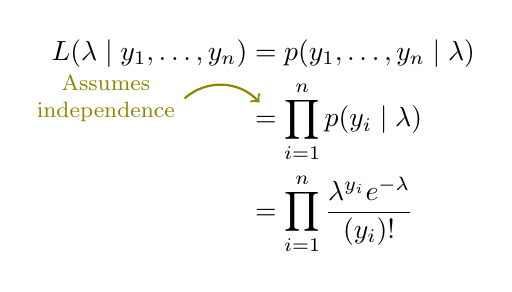
\begin{tikzpicture}
\node at (0,0) {$\begin{aligned}
L(\lambda\mid y_1,\dots,y_n) &= \pause p(y_1,\dots,y_n\mid \lambda) \\
&= \pause \prod_{i=1}^n p(y_i \mid \lambda) \\
&= \pause \prod_{i=1}^n \frac{\lambda^{y_i} e^{-\lambda}}{(y_i)!}
\end{aligned}$};
\onslide<3->{
	\node[olive, font = \footnotesize, align = center] (indep) at (-2,.6) {Assumes\\independence};
	\draw[olive,->, thick] (indep.east) to[bend left = 45] (-.05,.55);
}
\end{tikzpicture}
\end{center}
\end{frame}

\begin{frame}
What is the log likelihood? \pause
$$\begin{aligned}
\ell(\lambda \mid y_1,\dots,y_n) &= \pause \log L(\lambda\mid y_1,\dots,y_n) \\
&= \pause \sum_{i=1}^n \bigg(y_i\log \lambda - \lambda - \log(y_i!)\bigg) \\
&= \pause \log \lambda\sum_{i=1}^n y_i - n\lambda - \sum_{i=1}^n\log(y_i!) \\
&= \pause \underbrace{\log \lambda\sum_{i=1}^n y_i - n\lambda}_{\text{Involves }\lambda} - \underbrace{\sum_{i=1}^n\log(y_i!)}_{\text{Does not involve }\lambda} \\
&= \pause \log \lambda\sum_{i=1}^n y_i - n\lambda + \text{constant}
\end{aligned}$$
\end{frame}

\begin{frame}
What is the derivative of the log likelihood? \pause
$$\begin{aligned}
\frac{\partial}{\partial\lambda} \ell(\lambda\mid y_1,\dots,y_n) &= \frac{\partial}{\partial\lambda}  \log \lambda\sum_{i=1}^n y_i - n\lambda \\ \pause
&= \frac{1}{\lambda}\sum_{i=1}^n y_i - n
\end{aligned}$$ \pause
Set the derivative equal to 0 to find the critical value.
$$\begin{aligned}
0 &= \frac{1}{\lambda^*}\sum_{i=1}^n y_i - n \\ \pause
\lambda^* &= \frac{\sum_{i=1}^n y_i}{n}
\end{aligned}$$ \pause
Check second derivative is negative to verify this is a maximum. \pause
$$\frac{\partial^2}{\partial\lambda^2} \ell(\lambda\mid y_1,\dots,y_n) = -\frac{\sum_{i=1}^n y_i}{\lambda^2} < 0$$
\end{frame}

\begin{frame}
This is a maximum!
$$\hat\lambda_{\text{MLE}} = \frac{\sum_{i=1}^n y_i}{n}$$ \pause
Let's find the variance \pause

\begin{scriptsize}
$$\begin{aligned}
V(\hat\lambda_{\text{MLE}}) &= \bigg(\mathcal{I}_n(\lambda)\bigg)^{-1} \\
&= \pause \left(-E\left(\frac{\partial^2}{\partial\lambda^2}\ell(\lambda\mid y)\right)\right)^{-1} \\
&= \pause \left(-E\left(-\frac{\sum_{i=1}^n y_i}{\lambda^2}\right)\right)^{-1} \\
&= \pause \left(-\left(-\frac{\sum_{i=1}^n E(y_i)}{\lambda^2}\right)\right)^{-1} \\
&= \pause \left(-\left(-\frac{\sum_{i=1}^n \lambda}{\lambda^2}\right)\right)^{-1} \\
&= \pause \left(\frac{n \lambda}{\lambda^2}\right)^{-1} \\
&= \pause \frac{\lambda}{n} \\
\end{aligned}$$'
\end{scriptsize}
\end{frame}

\begin{frame}
This week is a lot of math. We appreciate the work you're putting in. \vskip 1cm \pause
We'll use this again and again and it will enable you to invent your own models in the future to fit your data generating processes! \vskip 1cm \pause
Keep it up! Also give us feedback on the cards.
\end{frame}

\section[Review: U of U]{Review: Universality of the Uniform}
\tcframe


\begin{frame}{Universality of the Uniform}{aka Probability Integral Transform, PIT}
\begin{theorem}
\begin{footnotesize}
\begin{itemize}
\item \normalfont Regardless of the distribution of $X$, $F(X)\sim \text{Uniform}(0,1)$
\item For a r.v. $X$ with CDF $F$ and a Uniform r.v. $U$, $F^{-1}(U)\sim X$
\end{itemize}
\end{footnotesize}
\end{theorem}
\begin{center}
\includegraphics<2| handout:2>[height = .6\textheight]{figs/UofUSims/sim1.pdf}
\includegraphics<3| handout:3>[height = .6\textheight]{figs/UofUSims/sim2.pdf}
\includegraphics<4| handout:4>[height = .6\textheight]{figs/UofUSims/sim3.pdf}
\includegraphics<5| handout:5>[height = .6\textheight]{figs/UofUSims/sim4.pdf}
\includegraphics<6| handout:6>[height = .6\textheight]{figs/UofUSims/sim5.pdf}
\includegraphics<7| handout:7>[height = .6\textheight]{figs/UofUSims/sim6.pdf}
\includegraphics<8| handout:8>[height = .6\textheight]{figs/UofUSims/sim7.pdf}
\includegraphics<9| handout:9>[height = .6\textheight]{figs/UofUSims/sim8.pdf}
\includegraphics<10| handout:10>[height = .6\textheight]{figs/UofUSims/sim9.pdf}
\includegraphics<11| handout:11>[height = .6\textheight]{figs/UofUSims/sim10.pdf}
\includegraphics<12| handout:12>[height = .6\textheight]{figs/UofUSims/sim11.pdf}
\includegraphics<13| handout:13>[height = .6\textheight]{figs/UofUSims/sim12.pdf}
\includegraphics<14| handout:14>[height = .6\textheight]{figs/UofUSims/sim13.pdf}
\includegraphics<15| handout:15>[height = .6\textheight]{figs/UofUSims/sim14.pdf}
\includegraphics<16| handout:16>[height = .6\textheight]{figs/UofUSims/sim15.pdf}
\includegraphics<17| handout:17>[height = .6\textheight]{figs/UofUSims/sim16.pdf}
\includegraphics<18| handout:18>[height = .6\textheight]{figs/UofUSims/sim17.pdf}
\includegraphics<19| handout:19>[height = .6\textheight]{figs/UofUSims/sim18.pdf}
\includegraphics<20| handout:20>[height = .6\textheight]{figs/UofUSims/sim19.pdf}
\includegraphics<21| handout:21>[height = .6\textheight]{figs/UofUSims/sim20.pdf}
\includegraphics<22| handout:22>[height = .6\textheight]{figs/UofUSims/sim21.pdf}
\includegraphics<23| handout:23>[height = .6\textheight]{figs/UofUSims/sim22.pdf}
\includegraphics<24| handout:24>[height = .6\textheight]{figs/UofUSims/sim23.pdf}
\includegraphics<25| handout:25>[height = .6\textheight]{figs/UofUSims/sim24.pdf}
\includegraphics<26| handout:26>[height = .6\textheight]{figs/UofUSims/sim25.pdf}
\includegraphics<27| handout:27>[height = .6\textheight]{figs/UofUSims/sim100.pdf}
\includegraphics<28| handout:28>[height = .6\textheight]{figs/UofUSims/sim500.pdf}
\includegraphics<29| handout:29>[height = .6\textheight]{figs/UofUSims/sim1000.pdf}
\includegraphics<30| handout:30>[height = .6\textheight]{figs/UofUSims/sim10000.pdf}
\end{center}
\end{frame}

\end{document}

%%%%% CUTTING THE SECTION BELOW %%%%%
\section[R2: Numeric integration]{Review 2: Numeric integration}
\tcframe

\begin{frame}
\Huge DRAFT: This section is a work in progress.
\end{frame}

\begin{frame}{Expected value as an integral}
\Huge

Key lesson: \vskip .5cm

\centering \blue{Analytic integration}\\is often \bgreen{hard}. \vskip .5cm
\blue{Numeric integration}\\in R is \bgreen{easy}!

\end{frame}

\begin{frame}{Expected value by analytic integration: Uniform}
$$E(X) = \pause \int_{-\infty}^\infty x f_X(x)\d x$$ \pause
Suppose $U\sim \text{Uniform(a,b)}$. \\
Remember the Uniform pdf is
$$f_U(u) = \begin{cases}
\frac{1}{b-a},& \text{if }u>a\text{ and }u<b \\
0,& \text{otherwise} \\
\end{cases}$$
Can we write the formula for $E(U)$? \pause
\begin{footnotesize}
\begin{center}
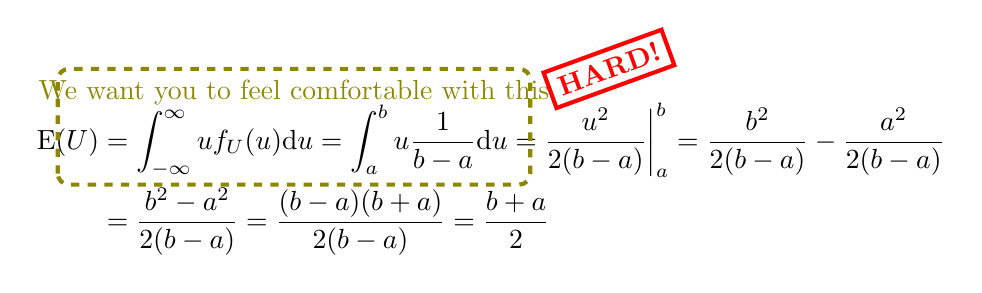
\begin{tikzpicture}
\node at (0,0) {$\begin{aligned}
\E(U) &= 
	\int_{-\infty}^\infty uf_U(u)\d u = 
	\pause \int_a^b u \frac{1}{b-a}\d u 
	\pause \pause = \frac{u^2}{2(b-a)}\bigg\rvert_{a}^b = 
	\pause \frac{b^2}{2(b-a)} - \frac{a^2}{2(b-a)} \\
	& = \pause \frac{b^2 - a^2}{2(b-a)} = 
	\pause \frac{(b-a)(b+a)}{2(b-a)} = \pause \frac{b+a}{2}
\end{aligned}$};
\onslide<6->{
\draw[line width = 1.5pt, rounded corners, dashed, olive] (-5.5,-.07) rectangle (.5,1.4);
\node[olive] at (-2.5, 1.1) {We want you to feel comfortable with this};
}
\onslide<7->{
\node[red,draw,rotate=20, line width = 1.5pt,font = \bf] at (1.5, 1.4) {HARD!};
}
\end{tikzpicture}
\end{center}
\end{footnotesize}
\end{frame}

\begin{frame}[fragile]{Expected value by numeric integration: Uniform}

\begin{center}
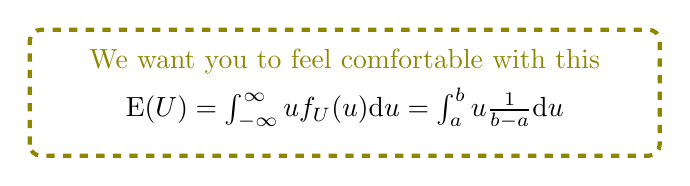
\begin{tikzpicture}
\node at (0,0) {$\E(U) = 
	\int_{-\infty}^\infty uf_U(u)\d u = \int_a^b u \frac{1}{b-a}\d u$};
\draw[line width = 1.5pt, rounded corners, dashed, olive] (-4,-.6) rectangle (4,1);
\node[olive] at (0, .6) {We want you to feel comfortable with this};
\end{tikzpicture}
\end{center}
If $a = 0$ and $b = 10$, \\
\begin{center}
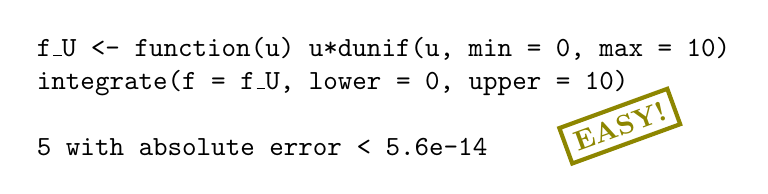
\begin{tikzpicture}
\node[align=left,anchor=south] at (0,0) {
\texttt{f\_U <- function(u) u*dunif(u, min = 0, max = 10)} \\
\texttt{integrate(f = f\_U, lower = 0, upper = 10)} \\ \\
\texttt{5 with absolute error < 5.6e-14}
};
\node[olive, draw, line width = 1.5pt, rotate=20, font = \bf] at (3,.5) {EASY!};
\end{tikzpicture}
\end{center}
\end{frame}

\begin{frame}[fragile]{Expected value by Monte Carlo integration: Uniform}

\begin{center}
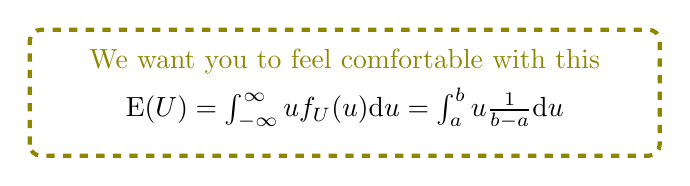
\begin{tikzpicture}
\node at (0,0) {$\E(U) = 
	\int_{-\infty}^\infty uf_U(u)\d u = \int_a^b u \frac{1}{b-a}\d u$};
\draw[line width = 1.5pt, rounded corners, dashed, olive] (-4,-.6) rectangle (4,1);
\node[olive] at (0, .6) {We want you to feel comfortable with this};
\end{tikzpicture}
\end{center}
If $a = 0$ and $b = 10$, \\
\begin{center}
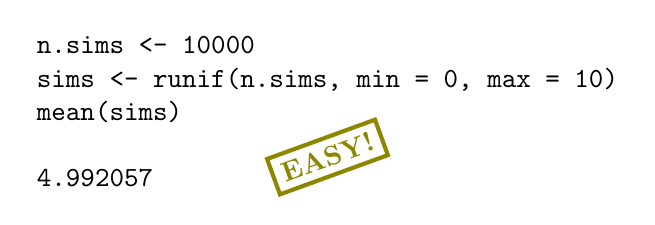
\begin{tikzpicture}
\node[align=left,anchor=south] at (0,0) {
\texttt{n.sims <- 10000} \\
\texttt{sims <- runif(n.sims, min = 0, max = 10)} \\
\texttt{mean(sims)} \\ \\
\texttt{4.992057}
};
\node[olive, draw, line width = 1.5pt, rotate=20, font = \bf] at (0,.5) {EASY!};
\end{tikzpicture}
\end{center}
\end{frame}

\begin{frame}{Expected value by analytic integration: Beta}
Suppose
$$f_Y(y) = \begin{cases} \frac{\Gamma(\alpha + \beta)}{\Gamma(\alpha)\Gamma(\beta)} y^{\alpha - 1}(1-y)^{\beta-1} &\qquad \text{for }y\in [0,1] \\
0 &\qquad \text{otherwise} \end{cases}$$ 
This is called the \href{https://en.wikipedia.org/wiki/Beta_distribution}{\textbf{beta distribution}}.  \\
\begin{tikzpicture}[x = .3\textwidth]
\node[anchor=east, align=center] at (0,0) {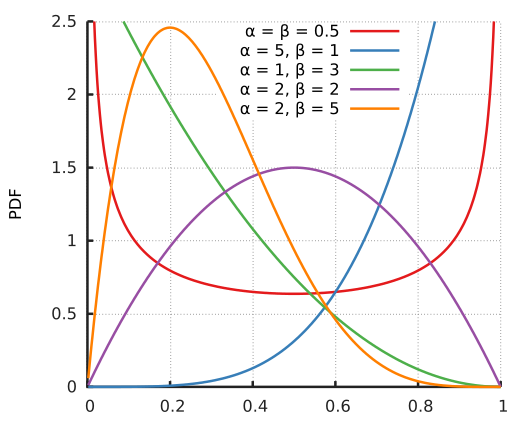
\includegraphics[width = .5\textwidth]{figs/beta}\\Image source: Wikipedia};
\node[anchor=west, align=left, font = \footnotesize] at (0,0) {
	\bgreen{Story:} If the wait time until a shooting \\
	star arrives is $X\sim \text{Exponential}(\lambda)$,\\
	then the wait time until $a$ shooting stars \\
	arrive is $G_a\sim \text{Gamma}(a,\lambda)$.\\
	If you wait for $\alpha + \beta$ shooting stars \\
	to arrive, the proportion of the total spent \\
	waiting for the first $\alpha$ stars \\
	is $B\sim \text{Beta}(\alpha,\beta)$.
};
\end{tikzpicture}
\end{frame}

\begin{frame}{Expected value by analytic integration: Beta}
\footnotesize
$$f_Y(y) = \begin{cases} \frac{\Gamma(\alpha + \beta)}{\Gamma(\alpha)\Gamma(\beta)} y^{\alpha - 1}(1-y)^{\beta-1} &\qquad \text{for }y\in [0,1] \\
0 &\qquad \text{otherwise} \end{cases}$$
\begin{center}
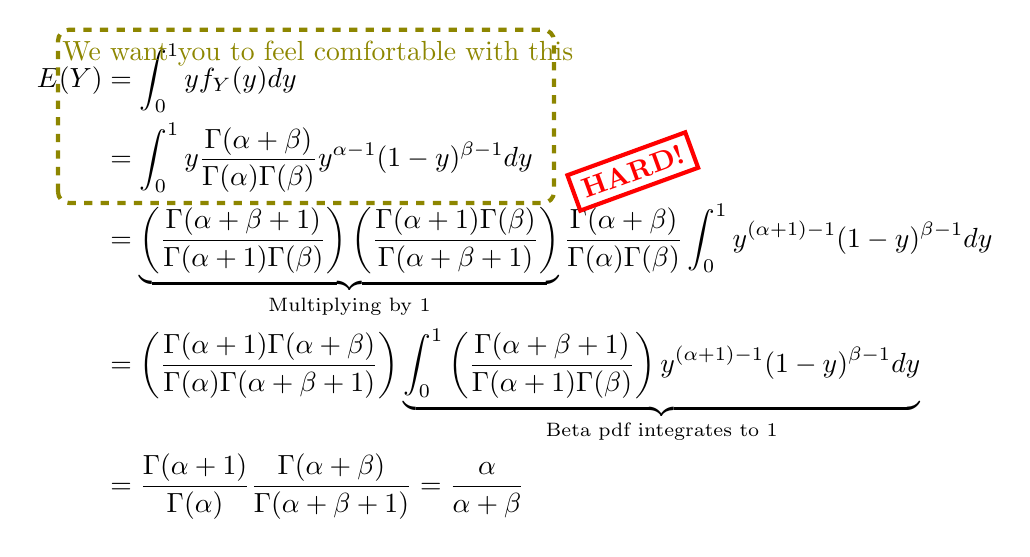
\begin{tikzpicture}
\node at (0,0) {$\begin{aligned}
E(Y) &= \pause \int_0^1 y f_Y(y)dy \\ 
&= \pause \int_0^1 y \frac{\Gamma(\alpha + \beta)}{\Gamma(\alpha)\Gamma(\beta)} y^{\alpha - 1}(1-y)^{\beta-1} dy \\ \pause \pause
&= \underbrace{\left(\frac{\Gamma(\alpha + \beta + 1)}{\Gamma(\alpha + 1)\Gamma(\beta)}\right)\left(\frac{\Gamma(\alpha + 1)\Gamma(\beta)}{\Gamma(\alpha + \beta + 1)}\right)}_{\text{Multiplying by 1}}\frac{\Gamma(\alpha + \beta)}{\Gamma(\alpha)\Gamma(\beta)} \int_0^1 y^{(\alpha+1) - 1}(1-y)^{\beta-1} dy \\ \pause
&= \left(\frac{\Gamma(\alpha + 1)\Gamma(\alpha + \beta)}{\Gamma(\alpha)\Gamma(\alpha + \beta + 1)}\right) \underbrace{\int_0^1 \left(\frac{\Gamma(\alpha + \beta + 1)}{\Gamma(\alpha + 1)\Gamma(\beta)}\right)y^{(\alpha+1) - 1}(1-y)^{\beta-1} dy}_{\text{Beta pdf integrates to 1}} \\ \pause
&= \frac{\Gamma(\alpha + 1)}{\Gamma(\alpha)}\frac{\Gamma(\alpha + \beta)}{\Gamma(\alpha + \beta + 1)} = \frac{\alpha}{\alpha + \beta}
\end{aligned}$};
\onslide<4->{
\draw[line width = 1.5pt, rounded corners, dashed, olive] (-5.8,1) rectangle (.5,3.2);
\node[olive] at (-2.5, 2.9) {We want you to feel comfortable with this};
}
\onslide<5->{
\node[red,draw,rotate=20, line width = 1.5pt,font = \bf] at (1.5, 1.4) {HARD!};
}
\end{tikzpicture}
\end{center}
\end{frame}

\begin{frame}[fragile]{Expected value by numeric integration: Beta}
\footnotesize
\begin{center}
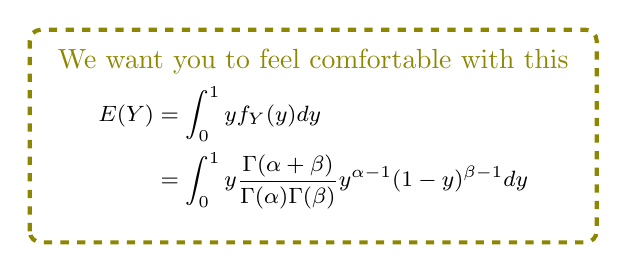
\begin{tikzpicture}
\node[font=\footnotesize] at (0,0) {$\begin{aligned}
E(Y) &= \pause \int_0^1 y f_Y(y)dy \\ 
&= \pause \int_0^1 y \frac{\Gamma(\alpha + \beta)}{\Gamma(\alpha)\Gamma(\beta)} y^{\alpha - 1}(1-y)^{\beta-1} dy
\end{aligned}$};
\draw[line width = 1.5pt, rounded corners, dashed, olive] (-3.6,-1.2) rectangle (3.6,1.5);
\node[olive] at (0, 1.1) {We want you to feel comfortable with this};
\end{tikzpicture}
\end{center}
\begin{small}
\begin{semiverbatim}
\pause
beta.pdf <- function(alpha,beta,y) \{
  gamma(alpha + beta) / (gamma(alpha) * gamma(beta)) *
    y^(alpha - 1) * (1 - y)^(beta - 1)
\}
\pause
integrate(f = function(y) y * beta.pdf(alpha = 1, beta = 2, y = y),
          lower = 0, upper = 1)
\pause
0.3333333 with absolute error < 3.7e-15
\end{semiverbatim}
\end{small}
\end{frame}

\begin{frame}[fragile]{Expected value by numeric integration: Beta}
\footnotesize
\begin{center}
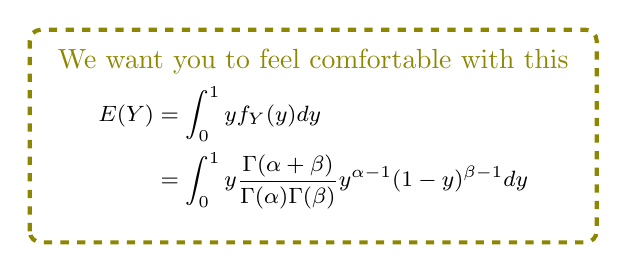
\begin{tikzpicture}
\node[font=\footnotesize] at (0,0) {$\begin{aligned}
E(Y) &= \pause \int_0^1 y f_Y(y)dy \\ 
&= \pause \int_0^1 y \frac{\Gamma(\alpha + \beta)}{\Gamma(\alpha)\Gamma(\beta)} y^{\alpha - 1}(1-y)^{\beta-1} dy
\end{aligned}$};
\draw[line width = 1.5pt, rounded corners, dashed, olive] (-3.6,-1.2) rectangle (3.6,1.5);
\node[olive] at (0, 1.1) {We want you to feel comfortable with this};
\end{tikzpicture}
\end{center}
\begin{small}
\begin{semiverbatim}
\pause
beta.pdf <- function(alpha,beta,y) \{
  gamma(alpha + beta) / (gamma(alpha) * gamma(beta)) *
    y^(alpha - 1) * (1 - y)^(beta - 1)
\}
\pause
integrate(f = function(y) y * beta.pdf(alpha = 1, beta = 2, y = y),
          lower = 0, upper = 1)
\pause
0.3333333 with absolute error < 3.7e-15
\end{semiverbatim}
\end{small}
\end{frame}

\begin{frame}{Variance as an integral}
$$\begin{aligned}
V(X) &= \pause E(X-E[X])^2 \\
&= \pause E(X^2) - (E[X])^2 \\
&= \pause \int_{-\infty}^\infty x^2 f_X(x)dx - \left(\int_{-\infty}^\infty x f_X(x)dx\right)^2
\end{aligned}$$
\end{frame}

\end{document}
